\chapter{Regularity of graphs and Ramsey's extremal theory}

As one can already met the random graphs which are denoted as $G = (n,p)$ where we have $n$ vertices and every edge between each pair of a vertices is there with a probability $p$. This notation si usually used for proving some properties that graphs tend to have for more vertices.

Example could be computing the number of triangles in the graph. To be exact we want to compute the expected number, so $\E [\text{number of triangle}] = p^3 \binom{n}{3}$. And also then we may use Chernoff's bound to get that $\Pr [|\text{number of triangles } - p^3 \binom{n}{3}| > \epsilon n^3] = e^{-\Theta(n^3)}$. In other words the probability that the number being way different is small.

In the next example and for further reading we will denote $e(A,B)$ as the number of edges between two subset of vertices $A, B \subseteq V$. In the probability case it is somewhat similiar to $p |A| |B|$. Which leads to the fact that $\Pr [|e(A,B) - p|A||B|| \geq \epsilon |A||B|] < e^{-\Theta(|A||B|)}$. If we would take $A, B$ such that $|A|, |B| \geq \delta n$ then there may be $\leq 4^n$ number of subsets.

Well the real graphs we may encounter do not have this nice property. So we will build a theory around that in fact it is not that bad and can be somewhat similiar to the probability case.

\begin{defn}
	Lets denote $d(A,B) = \frac{e(A,B)}{|A| \cdot |B|}$ or so called density of a graph. Sometimes we will denote $d(A,B)$ as $p$, because it will behave somewhat similarly as the probability.
\end{defn}

\begin{defn}
	For some $\delta, \epsilon > 0$. Let $A, B \subseteq V$ for some graph $G = (V,E)$. Then we say that $(A,B)$ is $(\delta, \epsilon)$-\textbf{regular pair} if following holds
	
	\begin{itemize}
		\item $\forall A' \subseteq A : |A'| \geq \delta |A|$,
		\item $\forall B' \subseteq B : |B'| \geq \delta |B|$ and
		\item $|d(A'B') - d(A,B)| \leq \epsilon$.
	\end{itemize}
	
	Sometimes we will shorten the notation to just $\epsilon$-regular pair.
\end{defn}

Now we will look at how many neighbors can be for some $v \in A$. To be exact we will denote $B_{0}$ the neighbors and we want to count these vertices for which $|B_{0}| \geq \delta |B|$. But we may see there are some degenerate vertices, but we will show it is not that many.

\begin{lemma}
	The number of vertices in $A$ such that $\deg_{B_{0}}v > (p + \epsilon |B_{0}|)$ is at most $\delta |A|$. And also the number of vertices in $B$ such that $\deg_{A_{0}}v < (p + \epsilon |A_{0}|)$ is at most $\delta |B|$.
\end{lemma}

\begin{proof}
	For contradiction denote $A_{0}$ as all such vertices in $A$ which have low number of neighbors. For the contradiction suppose $|A_{0}| \geq \delta |A|$. This result in the following.
	
	$$
	\begin{aligned}
		|d(A_{0}, B_{0}) - p| &\leq \epsilon \\
		 &= \left| \frac{e(A_{0},B_{0})}{|A_{0}| |B_{0}|} - p \right| \\
		 &= \left| \frac{\sum_{v \in A_{0}} \deg_{b_{0}}(v)}{|A_{0}| |B_{0}|} - p \right| \\
		 &= \left| \frac{|A_{0} (p+ \epsilon |B_{0}|)}{|A_{0}| |B_{0}|} - p \right| \\
		 &= \frac{|A_{0} (p+ \epsilon |B_{0}|)}{|A_{0}| |B_{0}|} - p = \epsilon
	\end{aligned}
	$$
	
	Which is a contradiction.
\end{proof}

Now we will denote $q(A,B)$ as the number of vertices $(v_1, v_2, v_3, v_4)$ forming a 4-cycle and $v_1 \neq v_3 \in A$ and $v_2 \neq v_4 \in B$. In the probability case we see that 

$$
\E [q(A,B)] = p^4 \binom{|A|}{2} \binom{|B|}{2} \cdot 4 \approx p^4 |A|^2 |B|^2 - O(n^3)
$$

One can be confused by the $4$ in there. That is because the way we defined it we count every 4-cycle four times.

\begin{lemma}
	For a graph $G$ and $A, B \subseteq V$ as an $(A, B)$ $\epsilon$-regular pair and $|A| = |B|$ we have following inequalities.
	
	$$
	(p^4 - 6 \epsilon)n^4 - 2n^3 \leq q(A,B) \leq (p^4 + 16 \epsilon) n^4
	$$
\end{lemma}

The exact constants are not that necessary, so they are picked somewhat randomly. We will prove only the lower bound. The other one is similiar.

\begin{proof}
	Lets put $A_{0} = \{ v \in A : \deg_{B} v < (p - \epsilon) n\}$. Which by the lemma we get $|A_{0}| \leq \epsilon n$. Now lets take $v_1 \in A \setminus A_{0}$. Now lets consider such $B_{v_1}$ (neighbors of $v_1$) for which $|B_{v_1}| \geq (p - \epsilon) n$. WLOG we may assume it is $\ge \epsilon n$, otherwise the lower bound is negative. Denote $A_{v_1} = \{v \in A  : \deg_{B_{v_1}} v < (p - \epsilon) |B_{v_1}|\}$. Also by the lemma $|A_{v_1}| \leq \epsilon n$. Now we choose $v_3 \in A \setminus A_{v_1}$.
	
	Now we may say that the number of 4-cycles is $\geq (1-\epsilon)n (1 - \epsilon)n ((p - \epsilon) |B_{v_1}|)62 - 2n^3$. Where the first $(1-\epsilon)n$ is for $v_1$ and the second for $v_3$, we multiply it by the choices from $B$ and subtract all wrong choices (choosing the same vertex more than once). Now this can be calculated.
	
	$$
	\begin{aligned}
		\text{number of 4-cycles} & = (1- \epsilon)^2 (p - \epsilon)^4 n^4 - 2n^3 \\
		&\geq (1-2\epsilon) (p^4 - 4\epsilon) n^4 - 2n^3 \\
		&\geq (p^4 - 6\epsilon) n^4 - 2n^3
	\end{aligned}
	$$
\end{proof}

Now we will try to use this even more for computing the number of triangles from $A,B,C$ which are all $\epsilon$-regular pairs. Also denote the number as $t(A,B,C)$ then the densities will be denoted as $p_{AB}, p_{BC}, p_{AC}$. Also we are interested only in those triangles $v_1, v_2, v_3$ where $v_1 \in A, v_2 \in B, v_3 \in C$. In the random graph it would be $p_{AB} p_{BC} p_{AC} n^3$. But we will show it is also similiar with regular pairs.

\begin{lemma}
	For $\epsilon$-regular pairs $(A,B), (B,C), (A,C)$ which are the same size $|A| = |B| = |C| = n$ where the densities $d(X,Y)$ are denoted by $p_{XY}$ (as before). The following bounds hold.
	
	$$
	p_{AB} p_{BC} p_{AC} n^3 - 10 n^3 \leq t(A,B,C) \leq p_{AB} p_{BC} p_{AC} n^3 + 10 \epsilon n^3
	$$
\end{lemma}

\begin{proof}
	Now we will show us the upper bound. Lets consider these sets:
	
	$$
	\begin{aligned}
		A_1 &= \{ v \in A : \deg_B v \geq (p_{AB} + \epsilon) n\} \quad |A_1| \leq \epsilon n \\
		A_2 &= \{ v \in A : \deg_C v \geq (p_{AC} + \epsilon) n\} \quad |A_2| \leq \epsilon n
	\end{aligned}
	$$
	
	Now we consider three separate cases for which set is used for the $v_1 \in A$.
	
	\begin{enumerate}[(i)]
		\item $v_1 \in A_1$ then $\epsilon |A_1| n^2 \leq \epsilon n^3$.
		\item $v_2 \in A_2$ similarly $\epsilon |A_2| n^2 \leq \epsilon n^3$.
		\item Last case is if $v_1 \in A \setminus (A_1 \cup A_2)$. We denote as $B_{v_1}$ and $C_{v_1}$ the neighbors of $v_1$ in $B$ and $C$ respectively. By the definition $|B_{v_1}| \leq (p_{AB} + \epsilon) n$ and  $|C_{v_1}| \leq (p_{AC} + \epsilon) n$. Therefore altogether $e(B_{v_1}, C_{v_1}) \leq (P_{BC} +\epsilon) |B_{v_1}| |C_{v_1}| \leq (p_{AB} p_{BC} p_{AC} + 7\epsilon) n^2$. So we may have at most $\epsilon n^2$ choices for $B_{v_1}$ and $C_{v_1}$.
	\end{enumerate}
	
	If we sum it all then the $t(A,B,C) \leq 2\epsilon n63 + n (\epsilon n^2 + \epsilon n^2 + (p  + 7\epsilon)n^2) = (p + 9 \epsilon)n^3$.
\end{proof}

Now with all of that we would like to see if we are able to partition the vertices of graph $G$ into such sets which are $\epsilon$-regular. At least we would like to try bounding the number of partitions for some $m$ and larger $M_\epsilon$ which will be bounded to $\epsilon$. Well we may see that it won't work this way, like for the graph known as \textbf{Half graph} which is shown in the picture \ref{half-graph}.

\begin{figure}[!ht] \centering
	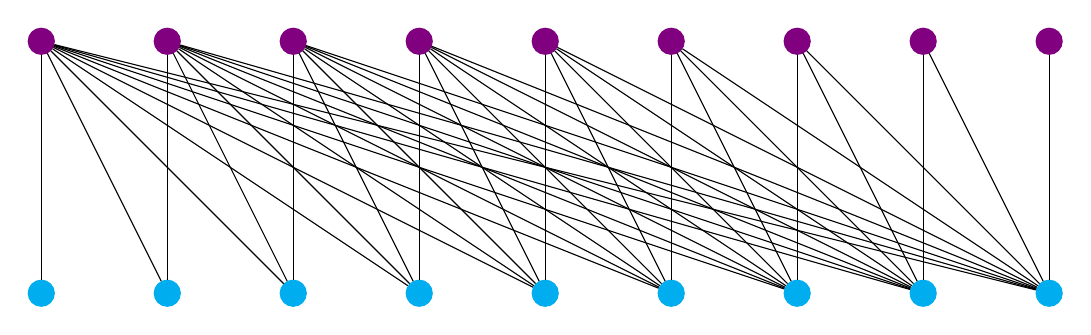
\begin{tikzpicture}[node distance={16mm}, main/.style = {draw, circle, fill}]
		\node[main, color=violet] (1) {};
		\node[main, right of = 1, color=violet] (2) {};
		\node[main, right of = 2, color=violet] (3) {};
		\node[main, right of = 3, color=violet] (4) {};
		\node[main, right of = 4, color=violet] (5) {};
		\node[main, right of = 5, color=violet] (6) {};
		\node[main, right of = 6, color=violet] (7) {};
		\node[main, right of = 7, color=violet] (8) {};
		\node[main, right of = 8, color=violet] (9) {};
		
		\node[below of = 1] (phantom) {};
		
		\node[main, below of = phantom, color=cyan] (11) {};
		\node[main, right of = 11, color=cyan] (12) {};
		\node[main, right of = 12, color=cyan] (13) {};
		\node[main, right of = 13, color=cyan] (14) {};
		\node[main, right of = 14, color=cyan] (15) {};
		\node[main, right of = 15, color=cyan] (16) {};
		\node[main, right of = 16, color=cyan] (17) {};
		\node[main, right of = 17, color=cyan] (18) {};
		\node[main, right of = 18, color=cyan] (19) {};
		
		\draw (1) edge (11) (1) edge (12)
			(1) edge (13) (1) edge (14)
			(1) edge (15) (1) edge (17)
			(1) edge (16) (1) edge (19)
			(1) edge (18);
			
		\draw (2) edge (12) (2) edge (13)
		    (2) edge (14) (2) edge (15)
		    (2) edge (17) (2) edge (16)
			(2) edge (19) (2) edge (18);
		
		\draw (3) edge (13) (3) edge (14)
			(3) edge (15) (3) edge (17)
			(3) edge (16) (3) edge (19)
			(3) edge (18);
			
		\draw (4) edge (14) (4) edge (15)
			(4) edge (17) (4) edge (16)
			(4) edge (19) (4) edge (18);
			
		\draw (5) edge (15) (5) edge (17)
			(5) edge (16) (5) edge (19)
			(5) edge (18);
			
		\draw (6) edge (17) (6) edge (16)
			(6) edge (19) (6) edge (18);
			
		\draw (1) (7) edge (17) (7) edge (19) (7) edge (18);
			
		\draw (8) edge (18) (8) edge (19);
			
		\draw  (9) edge (19);
	\end{tikzpicture}
	\caption{Counterexample of a graph $G$ as a half graph with $18$ vertices.}
	\label{half-graph}
\end{figure}

\begin{defn}
	We will denote $\epsilon$-regular partitioning of graph $G$ with $n = |V(G)|$ are disjoint parts $A_{1}, A_{2}, \dots, A_{k}$ of $V(G)$. When all properties are satisfied.
	
	\begin{enumerate}
		\item $|A_1| = |A_2| = \dots = |A_k|$,
		\item $|A_0| \leq \epsilon n$ and
		\item for $1 \leq i \leq j \leq m$, $(A_i, A_j)$ are $\epsilon$-regular with at most $\leq \epsilon m^2$ exceptions.
	\end{enumerate}
\end{defn}

\begin{thm}[Szemerédi, regularity lemma]
	$\forall \epsilon > 0, \forall m_0 \geq 1$ there exists $M$ such that $\forall G : |V(G)| \geq m_0$ there exists $\epsilon$-regular partitioning of $G$ $A_0, \dots, A_m$ that $m_0 \leq m \leq M$.
\end{thm}

This theorem may actually be useful in some other theoretical results but as we will show us later on the number $M$ is approximately

$$
2^{2{^{2^{2^{\reflectbox{$\ddots$}^{m_0}}}}}} \quad \text{where there is } \frac{1}{\epsilon^4} \text{ number of twos.}
$$